\section{Dokumentation und Metadaten}\label{ssc:Doku+Metadata}

Metadaten sind Daten über Daten. Metadaten sind dazu da, die eigentlichen Daten genauer zu beschreiben. Ein Druckwert alleine sagt nichts aus, es muss immer ein Kontext mit angegeben werden, an welchem System (z.B. in welchem Fluid) und an welcher Stelle gemessen wurde, mit welchem Drucksensor (Firma, Modell) und an welchem Messgerät war der Drucksensor angeschlossen, usw.

Die Dokumentation von Daten sowie die Erstellung von Metadaten sind unerlässlich, um Ihre Daten im Detail zu verstehen und auch anderen Forschenden zu helfen, Ihre Daten zu finden und weiter zu nutzen bzw. richtig zu zitieren. Damit werden Daten nachvollziehbar, ein wichtiger Aspekt für FAIR Data (siehe Kapitel \ref{ssc:FAIR-Data}).

Für die Erstellung von Metadaten gibt es bereits viele Vorlagen bzw. Metadaten-Standards bwz. -Schematas. Jede Disziplin hat eigene, fachspezifische Schemass, die Sie selber erfragen oder nachschlagen müssen. Falls es noch kein Schema für Ihr Gebiet oder Ihre Anwendung gibt, können selber Metadatenschema entworfen werden. Weitere allgemeine Leitlinien finden sie im folgenden Text.


\subsection{Wichtige Information beim Sammeln oder Erstellen von Daten}

\begin{itemize}
  \item Notieren Sie alle Dateinamen und -formate, die mit dem Projekt in
        Verbindung stehen, wie die Daten organisiert sind, wie die Daten
        erzeugt wurden (einschließlich aller verwendeten Geräte samt Software),
        und Informationen darüber, wie die Daten verändert oder verarbeitet
        wurden.
  \item Version und Hersteller von Messgeräten und Computerprogrammen (auch von den Steuerprogrammen der Messgeräte)
  \item Abkürzungen oder Variablen, die in den Daten oder in der Dateibenennungsstruktur verwendet werden.
\end{itemize}



\subsection{Dokumentation allgemeiner Daten im DataCite-Schema}\label{sc:data-documentation}

Am L-IWT wird ein weltweit verwendetes Metadatenschema verwendet zur Angabe von allgemeinen Metadaten. Unser Schema folgt den Empfehlungen des weltweiten DataCite-Konsor\-tiums (TIB Hannover, Britische Bibliothek, Denmark Technical Information Center, ETH Zürich, CalTech, Australian National Data Service, ...). Diese Metadaten können mithilfe unseres 'Readme File Creator' (siehe \ref{fig:readme-creator}) erzeugt und in einer "readme.json" Datei in \textbf{JEDEM VERZEICHNIS} Ihrer Daten gespeichert werden, um diese zu beschreiben. Alternativ
kann ieselbe DataCite-Metadaten-Struktur auch im JSON-Editor des ELNs (siehe \ref{ssc:ELN}) abgebildet bzw. eingegeben werden. \\
\begin{wrapfigure}{r}{0.5\linewidth}
  \vspace{-1em}
  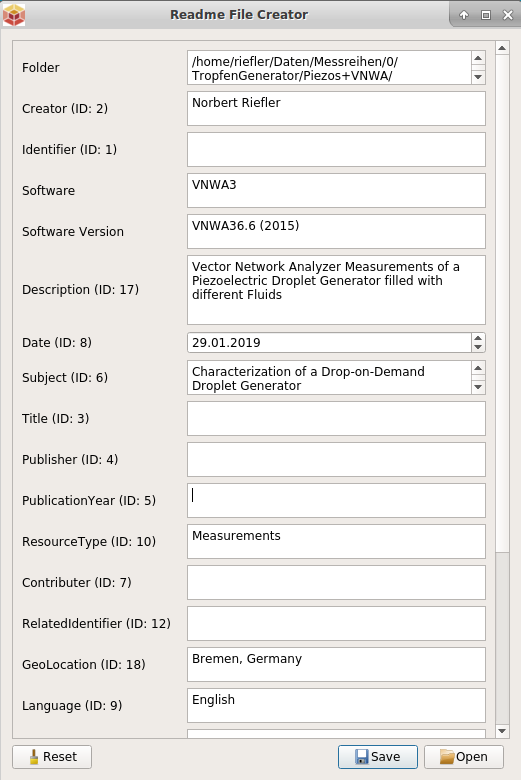
\includegraphics[width=\linewidth]{Figure02_ReadmeFileCreator.png}
  \caption{Data Input Tool: Readme-File-Creator}
  \label{fig:readme-creator}
\end{wrapfigure}
Im Folgenden werden einige der extrahierten Eigenschaften erläutert; weitere
Informationen finden Sie in Tabelle 3 in \cite{datacite2019}: \\[6pt]
%
\textbf{ID 1: Kennung} \\
Nummer, die zur Identifizierung der Daten verwendet wird. Dies kann ein DOI
(Digital Object Identifier) im Falle einer Veröffentlichung oder eine PID
(Persistent Identifier) aus dem ELN sein (eLabFTW  generiert eine lange Nummer
für jedes Experiment, siehe \ref{ssc:ELN} \nameref{ssc:ELN}). \\[6pt]
%
\textbf{ID 2: Erstellerin oder Ersteller} \\
Name der Person, die für die beschriebenen Daten verantwortlich ist (ORCID, Open Researcher Contributor Identification). \\[6pt]
%
\textbf{ID 3: Titel} \\
Kann der Titel eines Datensatzes, der Name einer Software oder der Titel eines
Artikels sein. \\[6pt]
%
\textbf{ID 4: Herausgeber} \\
Der Name der Einrichtung, die die Daten produziert, aufbewahrt, archiviert,
veröffentlicht, druckt, vertreibt, freigibt oder herausgibt (z.B.
"Leibniz-Institut für Werkstofforientierte Technologien - IWT"). \\[6pt]
%
\textbf{ID 5: Jahr der Veröffentlichung} \\
Das Jahr, in dem die Daten öffentlich zugänglich gemacht wurden oder werden. \\[6pt]
%
\textbf{ID 8: Datum} \\
Entstehungsdatum der Daten, einschließlich des Start- und Enddatums des
Projekts, des Datums der Datenänderung und des von den Daten abgedeckten. \\[6pt]
%
\textbf{ID 9: Sprache} \\
Sprache(n) des Inhalts der Quelle. \\[6pt]
%
\textbf{ID 10: Ressourcentyp} \\
Eine Beschreibung der Ressource; meist "DataSet", kann aber auch "\verb+Audiovisuell+",
"High-Speed Images", "DataPaper", etc. sein.\\[6pt]
%
\textbf{ID 19: Förderkennzeichen} \\
Organisationen oder Behörden, die die Forschung finanziert haben. \\[6pt]
%
\textbf{ID 16: Rechte} \\
Alle bekannten Rechte am geistigen Eigentum an den Daten. Die beste Wahl ist
normalerweise die Creative Commons Lizenz 'CC-BY' (BY attribution) oder 'CC-0'
für Daten sowie die 'CC Version 4.0' für schriftliche Dokumente. \\[6pt]
%
\textbf{ID 17: Beschreibung} \\
Wie die Daten erzeugt wurden, einschließlich der verwendeten Geräte oder
Software, des Versuchs\-protokolls und anderer Dinge, die Sie in ein Laborjournal
aufnehmen könnten. \\[6pt]
%
\textbf{ID 18: Geolokalisierung} \\
Wenn sich die Daten auf einen physischen Ort beziehen, halten Sie Informationen
über die geografische Abdeckung fest. \\[6pt]
%
Das oben in \autoref{fig:readme-creator} abgebildete Tool kann vom IWT-File-Server ($\rightarrow$Austausch $\rightarrow$Forschungs\-datenmanagement $\rightarrow$DataManagementGuidelines-ServiceFiles $\rightarrow$ReadmeFileCreator) für jedes Betriebssystem  heruntergeladen werden, um die Eingabe von Metadaten zu vereinfachen. Sie  können automatisch eine Datei namens 'readme.json' mit Ihren Metadaten, eingebettet in ein JSON (Java Scipt Object Notation)-Format, erstellen, die sowohl als Dokumentation als auch als Metadaten für Data Science Methods verwendet wird. Diese Datei wird in jedem Verzeichnis gespeichert, das Daten oder Programmcode enthält. Felder können einfach leer bleiben, wenn sie unzutreffend sind.\\
%
Dieselbe DataCite-Metadaten-Struktur kann auch im JSON-Editor des ELNs (siehe Kapitel \ref{ssc:ELN}) abgebildet bzw. eingegeben werden.


\subsection{Erzeugen eines Metadaten-Schema}
Ein Schema ist eine logische Struktur, die sowohl die Beziehungen zwischen den Metadaten-Elementen aufzeigt als auch Regeln für die Anwendung und Verwaltung der Metadaten liefert. Ein Beispiel für die Entwicklung eines Metadaten-Schema ist in der Arbeit von Eberskirch et al. \cite{elberskirch:2022} beschrieben, in der alle relevanten Parametern gesammelt wurden zur physikalischen als auch biologischen (toxikologischen) Charakterisierung von Nanopartikeln.
Die Entwicklung eines für die eigene Fachdisziplin passenden Schemas kann sehr hilfreich sein für die Strukturierung der Daten und des eigenen Wissens.






